\documentclass{jsarticle}
\usepackage[dvipdfmx]{hyperref}
\usepackage[dvipdfmx]{graphicx}
\usepackage{amssymb,amsmath,amsthm}
\usepackage{listings,jlisting}
\usepackage{newtxtt}
\usepackage{cases}
\usepackage[utf8]{inputenc}

\date{\today}
\author{山田龍}
\title{}
\begin{document}
\maketitle
\section{課題1}
まず、関数$f(t)$が、
\begin{numcases}
  {}
  -1 + 2t/\pi (0\leq t \leq \pi)& \\
  3 - 2t/\pi (\pi\leq t \leq 2\pi) &
\end{numcases}
と与えられるとき、フーリエ係数を解析的に求める。
フーリエ係数は、
\begin{align}
    c_k &= \frac{1}{T}\int f(t) e^{-i \frac{2 \pi kt}{T}}dt\\
    &= \frac{1}{2\pi}\int^{\pi}_{0}(-1 + 2t/\pi) e^{-ikt} dt
     + \frac{1}{2\pi}\int^{2\pi}_{\pi}(3 - 2t/\pi) e^{-ikt} dt\\
\end{align}
いま、$te^{-ikt}$の不定積分が
\begin{align}
    \int te^{-ikt} &= \left[ - \frac{te^{-ikt}}{ik}\right] + \int \frac{1}{ik}e^{-ikt}dt + C\\
         &= \left[ - \frac{te^{-ikt}}{ik}\right] + \frac{1}{k^2}\left[e^{-ikt}\right] + C\\
\end{align}
であることを使えば、
\begin{align}
    2\pi c_k &= \left[\frac{e^{-ikt}}{ik}\right]^{\pi}_0
    + \frac{2}{\pi}\left[ - \frac{te^{-ikt}}{ik}\right]^{\pi}_0
    + \frac{2}{\pi}\frac{1}{k^2}\left[e^{-ikt}\right]^{\pi}_0 
    - 3\left[\frac{e^{-ikt}}{ik}\right]^{2\pi}_{\pi}
    + \frac{2}{\pi}\left[\frac{te^{-ikt}}{ik}\right]^{2\pi}_{\pi}
    - \frac{2}{\pi}\frac{1}{k^2}\left[e^{-ikt}\right]^{2\pi}_{\pi}\\
    &= \frac{e^{-ik\pi} - 1}{ik}
    - \frac{2}{\pi}\frac{\pi e^{-ik\pi}}{ik}
    + \frac{2}{\pi}\frac{e^{-ik\pi} - 1}{k^2} 
    - 3\frac{e^{-ik2\pi} - e^{-ik\pi}}{ik}
    + \frac{2}{\pi}\frac{2\pi e^{-ik2\pi} - \pi e^{-ik\pi}}{ik}
    - \frac{2}{\pi}\frac{e^{-ik2\pi} - e^{-ik\pi}}{k^2}\\
    &= \frac{(-1)^k - 1}{ik}
    - 2\frac{(-1)^k}{ik}
    + \frac{2}{\pi}\frac{(-1)^k - 1}{k^2} 
    - 3\frac{1 - (-1)^k}{ik}
    + 2\frac{2 - (-1)^k}{ik}
    - \frac{2}{\pi}\frac{1 - (-1)^k}{k^2}\\
    &= \frac{2}{\pi}\frac{(-1)^k - 1}{k^2} 
    - \frac{2}{\pi}\frac{1 - (-1)^k}{k^2}\\
    &= \frac{2}{\pi k^2} ((-1)^k - 1 - 1 + (-1)^k)\\
    &= \frac{4}{\pi k^2} ((-1)^k - 1)\\
    \therefore c_k &= \frac{2}{\pi^2 k^2} ((-1)^k - 1)
\end{align}
解析解が求められた。次に
\begin{equation}
    f_N(t) = \sum^N_{-N} c_k e^{ikt}
\end{equation}
を使って$f_N$を計算した結果を図示すると以下\ref{f1}のようになる。
\begin{figure}[htbp]\label{f1}
    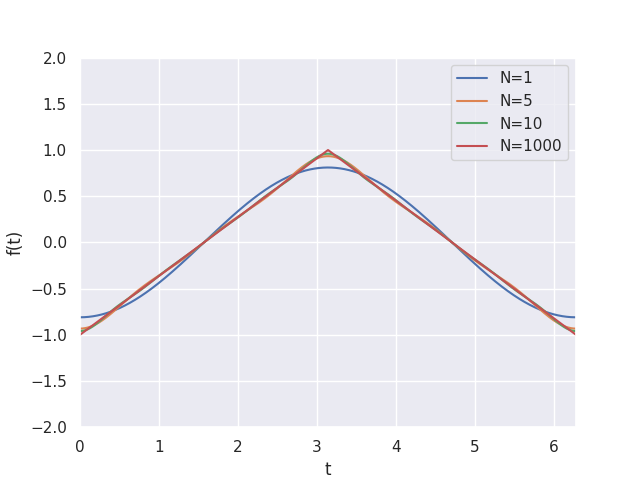
\includegraphics[clip,width=10.0cm]{./fourier_case1.png}
    \caption{$f_N$が$f(t)$の分布に近づく様子}
\end{figure}
また、誤差$f(t) - f_N(t)$の$N$依存性は以下\ref{f2}のようになる。
この図から、誤差は$N$の増大とともに急激に消えることがわかる。
右側のプロットは両対数グラフであるが、傾きから$f(t) - f_N(T) \propto N^{-2}$であることがわかる。
\begin{figure}[htbp]\label{f2}
    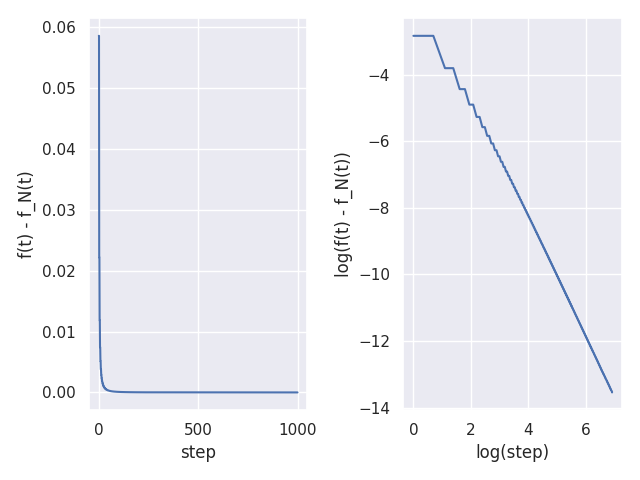
\includegraphics[clip,width=10.0cm]{./fourier_error_case1.png}
    \caption{誤差}
\end{figure}
\bibliographystyle{junsrt}
\bibliography{cite}
\end{document}